\documentclass{article}

% packages
\usepackage{amsmath,amssymb}
\usepackage{graphicx}
\usepackage{geometry}
\usepackage{enumerate}
\usepackage{setspace}


% definitions
\newtheorem{thm}{Theorem}
\newtheorem{df}{Definition}
\newtheorem{f}{Fact}
\newtheorem{lm}{Lemma}
\newtheorem{co}{Corrollary}

%commands
\newcommand{\X}{\mathbf{X}}
\newcommand{\W}{\mathbf{W}}
\newcommand{\E}{\text{ E}}
\newcommand{\C}{\text{ Cov}}
\newcommand{\B}{\mbox{\boldmath$\beta$}}
\newcommand{\G}{\mbox{\boldmath$\gamma$}}
\newcommand{\M}{\mbox{\boldmath$\mu$}}
\newcommand{\Si}{\mbox{\boldmath$\Sigma$}}
\newcommand{\sig}{\mbox{\boldmath$\sigma$}}
\newcommand{\ep}{\mbox{\boldmath$\varepsilon$}}
\newcommand{\V}{\text{ Var}}
\newcommand{\iid}{\overset{\text{iid}}{\sim}}
\newcommand{\ba}{\begin{array}}
\newcommand{\ea}{\end{array}}
\newcommand{\lp}{\left(}
\newcommand{\rp}{\right)}
\newcommand{\mb}{\mathbf}
\newcommand{\x}{\times}
\newcommand{\la}{\lambda}
\newcommand{\Proof}{\underline{Proof:}\\}
\newcommand{\inv}{^{-1}}
\newcommand{\bz}{\mb{z}}
\newcommand{\by}{\mb{y}}
\newcommand{\bx}{\mb{x}}
\newcommand{\boa}{\mb{a}}
\newcommand{\bob}{\mb{b}}
\newcommand{\bm}{\left[ \ba}
\newcommand{\fm}{\ea \right]}
\newcommand{\conas}{\overset{\text{a.s.}}{\to}}
\newcommand{\cond}{\overset{\text{d}}{\to}}
\newcommand{\conp}{\overset{\text{p}}{\to}}
\newcommand{\real}{\mathbb{R}}
\newcommand{\bX}{\mb{X}}
\newcommand{\bY}{\mb{Y}}
\newcommand{\bW}{\mb{W}}
\newcommand{\bZ}{\mb{Z}}

\title{Post Secondary Education Descriptive Statistics}
\author{Martin Guyer,  Feifei  Lei \\ Bin Zhuo, Kalbi Zongo}
\date{April 21, 2014}


\begin{document}

\maketitle

\section{Overview}

The \emph{United States Census Bureau} performs an ongoing yearly survey called the \textbf{American Community
Survey} to gather information about a variety of characteristics. These characteristics range from physical characteristics
like race, age, disabilities, etc, and environmental characteristics such as education level, income, employment status, etc. 
The main focus of these data is to provide the government with enough information to make educated decisions about 
programs and funding that is optimal for the American society. 

All of the students present today have made a decision to continue their education beyond secondary school. Therefore,
we see education as a valuable asset in our lives. The desire of the rest of this paper is to present the value of this asset and
how attainable it is for the many different races that populate the United States. As researchers we would like to answer 
three specific questions:
	\begin{enumerate}
	\item What percentage of people have attained some sort of post-secondary education in each of the fifty states?
	
	\item For each of the different races what proportion of people
  attain each of the different levels of post secondary education? 
	
	\item Which of these educational degrees has the highest average salary for each state?
	\end{enumerate}
These questions will allow us to better understand the value of education both by willingness of the United States
population to attain post-secondary educational degrees and the amount of money that companies are paying
those people with higher education degrees. 

\section{Findings}

Firstly, it is important to understand that each state does not value post-secondary education equally. We found that
the Northeastern United States contained the highest proportions of people that have received post-secondary
degrees, Massachusetts leading the group with over $30\%$ of its population having attained at least a bachelor's
degree. In contrast, the Southern states had the smallest proportion of people with post-secondary degrees. Arkansas had
the smallest amount of any state with only around $10\%$. This difference in the proportion of people who attain post-secondary
education could be indicative of the number of post-secondary institutions that a state has to offer these degrees to its
citizens. It could also indicate the number of jobs that the state has the require post-secondary education for entry level
positions. 

\begin{figure}
\includegraphics{StateHighEd.png}
\caption{In this figure, the darker the state the lower the proportion of people who attain a post-secondary degree. 
These degrees are: an associate's, a bachelor's, a master's degree, a professional degree, and a doctorate.}
\end{figure}

Upon investigating the proportion of each race that attains a post-secondary degree, the Asian race had the highest
proportion of people with between ($.25, .5$), in all of the states. Whereas, the people who identified themselves with
a tribe or with American Indians ranged between ($.05, .25$). These values may not be an indication of how much
a race values post-secondary education but the amount of opportunities that the race has to attain these degrees 
and become employed in a job where they can utilize their education. 

Therefore, we need to investigate how much people make who have attained these post-secondary education
degrees. Firstly, the table of the mean for all states is:
	\begin{center}
	\begin{tabular}{| l | r |} \hline
	Educational Level & Salary \\ \hline
	Associates & $ \$ 28,069.23$ \\
	Bachelor's & $ \$ 39,151.61$ \\
	Master's & $ \$ 47,484.37$ \\
	Professional & $ \$ 85,295.06$\\
	Doctorate & $ \$ 65,239.81$ \\ \hline
	\end{tabular}
	\end{center}
We can see that our country on average pays people with a professional degree much higher than any other
post-secondary educational level. This is understandable because professional degrees are attained for the benefit of
higher pay from companies. It would also be interesting to see, of the degrees that are not professional,
which educational level has the highest mean income in each state.  As can be seen in the following figure, people who
have a Professional degree have the highest average salary for all states. Also, the figure indicates that when we exclude
Professional degrees the highest average salary are for people who have a doctorate degree. 

\begin{figure}
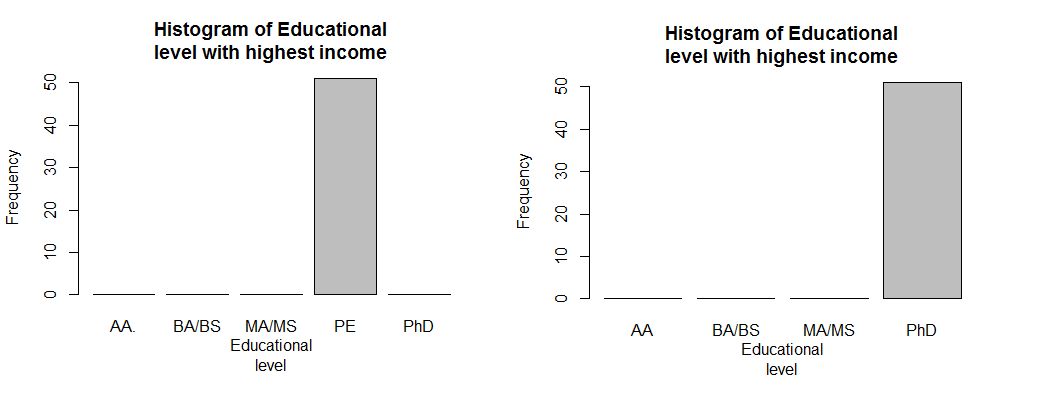
\includegraphics[scale=.55]{SalaryMaxes.png}
\caption{In this figure, we have two histograms. The histograms are of the number of states where the maximum income
was found in each of the post-secondary educational levels. It is apparent that professional degrees receive the highest
pay in all states. The second histogram indicates that excluding professional degrees, all states' highest average income is
for PhD's.}
\end{figure}

Therefore, given that the value of a degree is equal to the amount of money that it can earn you,
a Professional degree is the most valuable. Also, the more education that you have and degrees that you attain through 
academic study (excluding professional degrees) the higher your salary will most likely be throughout your life.  All in all, education
is extremely valuable and it would benefit all of us to continue our education both in school and the workforce by continually
attaining higher post-secondary degrees. 


\section{Obstacles and Solutions}

As with all data analysis, the largest amount of time is spent in the data manipulation and clean up step. This 
analysis was no different. In order to analyze the entire country, we needed to combine multiple large data sets into a
single file to be analyzed. Due the amount of different characteristics observed for each individual the first step was to 
reduce each of these files to only include the columns that were needed to answer our questions. The identification of 
each of the variables needed was to find its column identifier and the meaning of the codes that each number represented
found in \underline{2011 ACS PUMS Data Dictionary}. Using command lines, we were able to cut out columns and combine 
the four smaller datasets into one large complete dataset. 

After creating the dataset that needed to be analyzed it was operated on using different \textbf{dplyr} commands to 
optimize performance and relay only the results desired. We used commands such as \texttt{table\_df()}, \texttt{filter()},
 \texttt{summarize()}, \texttt{mutate()}, and \texttt{group\_by()} from \textbf{dplyr} accompanied with user defined
  functions to give proportions for each race. Obtaining the different numerical values was very quick and painless using
  \textbf{dplyr}. The real problem came with finding the proper way to graphically display the data.

\section{Future Questions/Work}

In this summary, we only present two different ways that the value of education can be shown through proportion
of those who attained these levels of education and the monetary value that companies give to those who have these
levels of education. These are only two ways that one can see the value of education. It would be important to further
understand the benefits of continuing ones education in the American society. There are also possible drawbacks to 
post-secondary educational achievements, which were not presented or analyzed. 

A more full understanding of the values of education would be found through researching other characteristics of those
who continue their education past secondary school and trying to find out both the positive and negative characteristics
that each level of education has. Also, it is important to note that all of the findings here are only correlated relationships and 
there is no proof of causation. Therefore, it could be an important experiment for social scientists to try to find out if there
is not just correlation but causation between these characteristics and level of educational attainment. 

\end{document}
